\chapter{Structure of a PASS Description}
	In this chapter we describe the structure of a PASS specification. The structure of a PASS descritption consists of the subjects and the messages they exchange.

\section{Informal Description}
\subsection{Subject}

Subjects are the active entities in system described in PASS in dependent how they are implemented. Subjects can be relized either by human, machines, software all combinitions of them. Subject descriptions do not contain any information about their implementation. If implementaion information is added to a subject it becomes an actor.\
In the following we use aan example for the informal definiton of subjects.\
In the simple scenario of the business trip application, we can identify three subjects, namely the employee as applicant, the manager as the approver, and the travel office as the travel arranger.

The definition of which subjects should be part of a process is a leadership decision. On the one hand, the necessary subjects result from the actual (as-is) situation, as it has for example already been described in the process analysis. On the other hand, the subject scoping, i.e., the question of what subjects there are and what tasks they roughly perform, can be adjusted to the envisioned or desired (to-be) situation.

Depending on the required or desired division of labor in a process, a corresponding number of subjects is necessary. This division is a design decision that must be taken in accordance with business needs. It influences the necessary granularity of a process model (see Section XXXXX).

In case there are many specialized subjects involved in a process, it may lead to many potentially complex interactions between the subjects. This can be a problem, since the communication between process participants always carries the risk of delays and misunderstandings. In case of few subjects, however, the subject carriers often cover a too wide a range of activities, which puts high demands on the participants. The decision with respect to subject scoping therefore has far-reaching consequences. It is complex, represents a major challenge, and requires extensive experience and care.

There are the following types of subjects:
\begin{itemize}
	\item Fully specified subjects \\
	This is the standard subject type. A subject communicates with other subjects by exchangeing messages.
	\item Multisubjects \\
	Multisubjects are simular to Fully specified subjects. If in a process model several identical subjects are required e.g. in order to increse the through put these subjects can be modelled by a multi subject. If several communicating subjects in a process modell are multi subjects they can be combined to a multi process 
	\item Single subject
	\item Interface subjects \\
\end{itemize}


\subsubsection{Fully specified Subjects}
Received messages
Send messages
Data
Input Pool

\subsubsection{Multsubjects and Multiprocesses}

\subsubsection{Single subjects}

\subsubsection{Interface Subjects}


\subsection{Subject-to-Subject Communication}
After the identification of subjects involved in the process (as process-specific roles), their interaction relationships need to be represented. These are the messages exchanged between the subjects. Such messages might contain structured information—so-called business objects (see Section xxxxxxx).\

The result is a model structured according to subjects with explicit communication relationships, which is referred to as a Subject Interaction Diagram (SID) or, synonymously, as a Communication Structure Diagram (CSD) (see \figurename{fig:beispiel-subject-interaction}).

\begin{figure*}
	\centering
	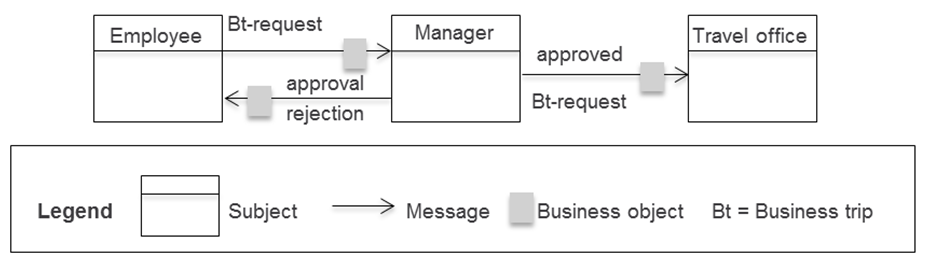
\includegraphics[width=14cm]{20181026-Ontologie-Bilder/Grafiken-Ontologie/SUbject-Interaction/Beispiel-Subject-Interaction}
	\caption[Subject interaction diagram]{Subject interaction diagram for the process ‘business trip application’}
	\label{fig:beispiel-subject-interaction}
\end{figure*}


Messages represent the interactions of the subjects during the execution of the process. We recommend naming these messages in such a way that they can be immediately understood and also reflect the meaning of each particular message for the process. In the sample ‘business trip application’, therefore, the messages are referred to as ‘business trip request’, ‘rejection’, and ‘approval’.

Messages serve as a container for the information transmitted from a sending to a receiving subject. There are two options for the message content:

\begin{itemize}
	\item 	Simple data types: Simple data types are string, integer, character, etc. In the business trip application example, the message ‘business trip request’ can contain several data elements of type string (e.g., destination, reason for traveling, etc.), and of type number (e.g., duration of trip in days).
	\item Business Objects: Business Objects in their general form are physical and logical ‘things’ that are required to process business transactions., We consider data structures composed of elementary data types, or even other data structures, as logical business objects in business processes. For instance, the business object ‘business trip request’ could consist of the data structures ‘data on applicants’, ‘travel data’, and ‘approval data’—with each of these in turn containing multiple data elements.
\end{itemize}


\subsection{Message Exchange}

In the previous subsection, we have stated that messages are transferred between subjects and have described the nature of these messages. What is still missing is a detailed description of how messages can be exchanged, how the information they carry can be transmitted, and how subjects can be synchronized. These issues are addressed in the following sub-sections.

\subsubsection{Synchronous and Asynchronous Exchange of Messages}
In the case of synchronous exchange of messages, sender and receiver wait for each other until a message can be passed on. If a subject wants to send a message and the receiver (subject) is not yet in a corresponding receive state, the sender waits until the receiver is able to accept this message. Conversely, a recipient has to wait for a desired message until it is made available by the sender.\

The disadvantage of the synchronous method is a close temporal coupling between sender and receiver. This raises problems in the implementation of business processes in the form of workflows, especially across organizational borders. As a rule, these also represent system boundaries across which a tight coupling between sender and receiver is usually very costly. For long-running processes, sender and receiver may wait for days, or even weeks, for each other.\

Using asynchronous messaging, a sender is able to send anytime. The subject puts a message into a message buffer from which it is picked up by the receiver. However, the recipient sees, for example, only the oldest message in the buffer and can only accept this particular one. If it is not the desired message, the receiver is blocked, even though the message may already be in the buffer, but in a buffer space that is not visible to the receiver. To avoid this, the recipient has the alternative to take all of the messages from the buffer and manage them by himself. In this way, the receiver can identify the appropriate message and process it as soon as he needs it. In asynchronous messaging, sender and receiver are only loosely coupled. Practical problems can arise due to the in reality limited physical size of the receive buffer, which does not allow an unlimited number of messages to be recorded. Once the physical boundary of the buffer has been reached due to high occupancy, this may lead to unpredictable behavior of workflows derived from a business process specification. To avoid this, the input-pool concept has been introduced in PASS.


\subsubsection{Exchange of Messages via the Input Pool}
To solve the problems outlined in asynchronous message exchange, the input pool concept has been developed. Communication via the input pool is considerably more complex than previously shown; however, it allows transmitting an unlimited number of messages simultaneously. Due to its high practical importance, it is considered as a basic construct of PASS.
Consider the input pool as a mail box of work performers, the operation of which is specified in detail.
Each subject has its own input pool. It serves as a message buffer to temporarily store messages received by the subject, independent of the sending communication partner. The input pools are therefore inboxes for flexible configuration of the message exchange between the subjects. In contrast to the buffer in which only the front message can be seen and accepted, the pool solution enables picking up (= removing from the buffer) any message. For a subject, all messages in its input pool are visible.

The input pool has the following configuration parameters (see \figurename{Figure 5.2}):
\begin{itemize}
	\item Input-pool size: The input-pool size specifies how many messages can be stored in an input pool, regardless of the number and complexity of the message parameters transmitted with a message. If the input pool size is set to zero, messages can only be exchanged synchronously.
	\item Maximum number of messages from specific subjects: For an input pool, it can be determined how many messages received from a particular subject may be stored simultaneously in the input pool. Again, a value of zero means that messages can only be accepted synchronously.
	\item Maximum number of messages with specific identifiers: For an input pool, it can be determined how many messages of a specifically identified message type (e.g., invoice) may be stored simultaneously in the input pool, regardless of what subject they originate from. A specified size of zero allows only for synchronous message reception.
	\item Maximum number of messages with specific identifiers of certain subjects: For an input pool, it can be determined how many messages of a specific identifier of a particular subject may be stored simultaneously in the input pool. The meaning of the zero value is analogous to the other cases.
\end{itemize}

\begin{figure}[ph]
	\centering
	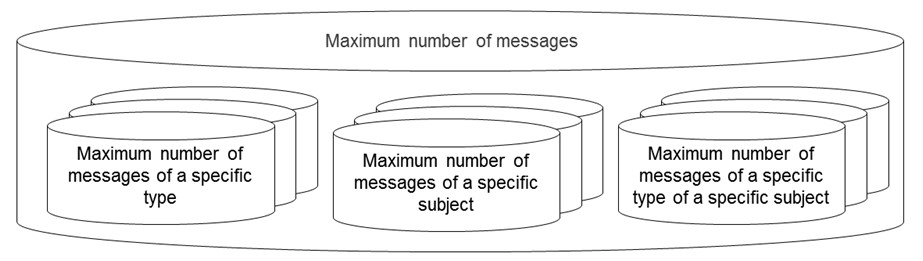
\includegraphics[width=14cm]{20181026-Ontologie-Bilder/Grafiken-Ontologie/SUbject-Interaction/input-pool-informal.jpg}
	\caption[Input Pool]{Configuration of Input Pool Parameters}
	\label{fig:input-pool}
\end{figure}


By limiting the size of the input pool, its ability to store messages may be blocked at a certain point in time during process runtime. Hence, messaging synchronization mechanisms need to control the assignment of messages to the input pool. Essentially, there are three strategies to handle the access to input pools:
\begin{itemize}
	\item Blocking the sender until the input pool’s ability to store messages has been reinstated: Once all slots are occupied in an input pool, the sender is blocked until the receiving subject picks up a message (i.e. a message is removed from the input pool). This creates space for a new message. In case several subjects want to put a message into a fully occupied input pool, the subject that has been waiting longest for an empty slot is allowed to send. The procedure is analogous if corresponding input pool parameters do not allow storing the message in the input pool, i.e., if the corresponding number of messages of the same name or from the same subject has been put into the input pool.
	\item Delete and release of the oldest message: In case all the slots are already occupied in the input pool of the subject addressed, the oldest message is overwritten with the new message.
	\item Delete and release of the latest message: The latest message is deleted from the input pool to allow depositing of the newly incoming message. If all the positions in the input pool of the addressed subject are taken, the latest message in the input pool is overwritten with the new message. This strategy applies analogously when the maximum number of messages in the input pool has been reached, either with respect to sender or message type.
\end{itemize}

\newpage

\section{OWL Description}

\subsection{Subject Interaction}

\begin{figure*}[ph]
	\centering
	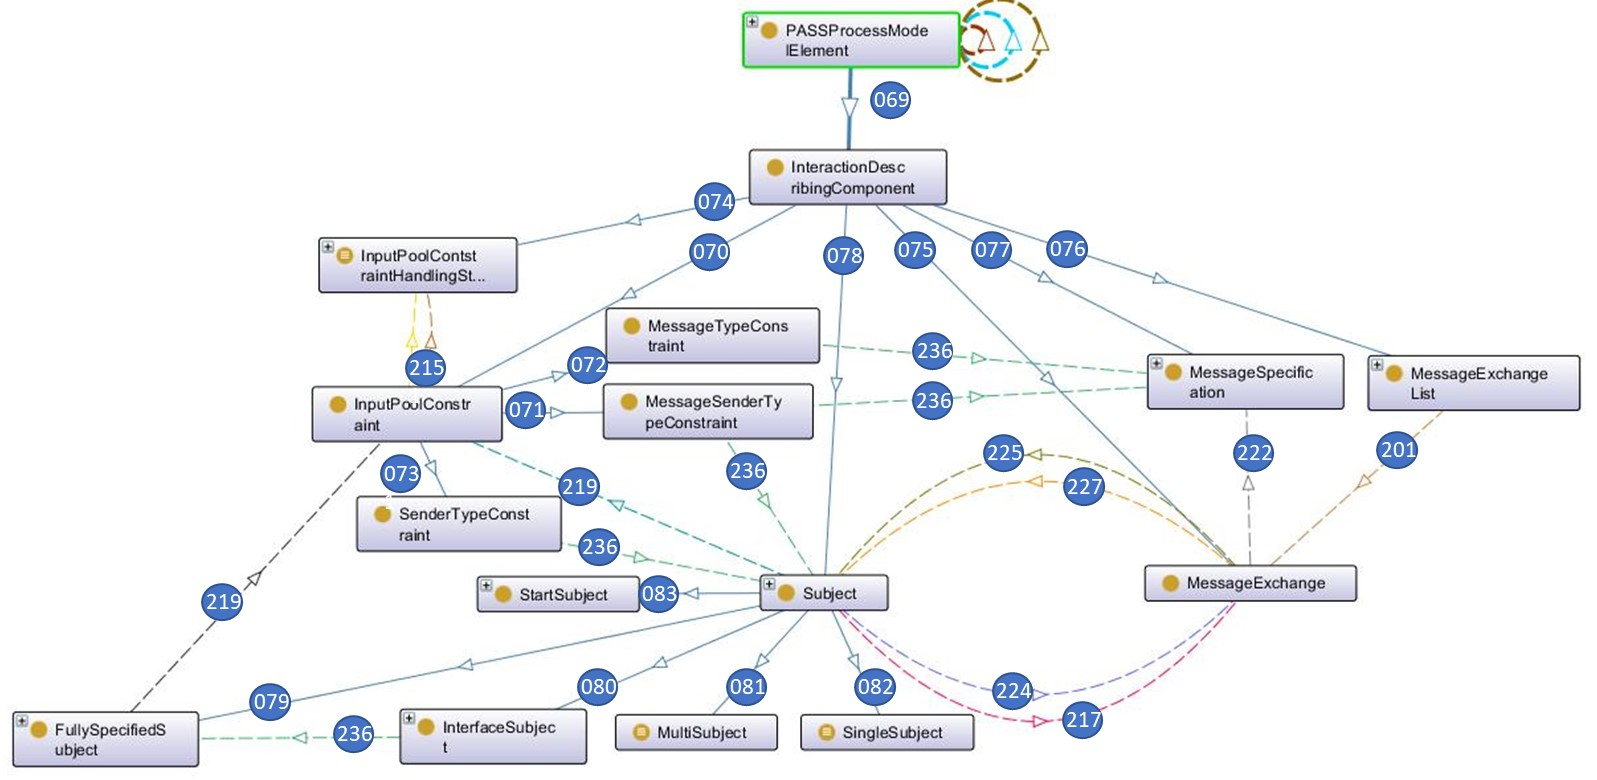
\includegraphics[width=16cm]{20181026-Ontologie-Bilder/Grafiken-Ontologie/SUbject-Interaction/OntoGrSubjectInteraction}
	\caption[Sructure of Subject Interactions]{Sructure of Subject Interactions}
	\label{fig:ontogrsubjectinteraction}
\end{figure*}







\newpage

\subsection{Subjects}

Different types of subjects \ref{fig:20181205-subject}
\begin{figure}[ph]
	\centering
	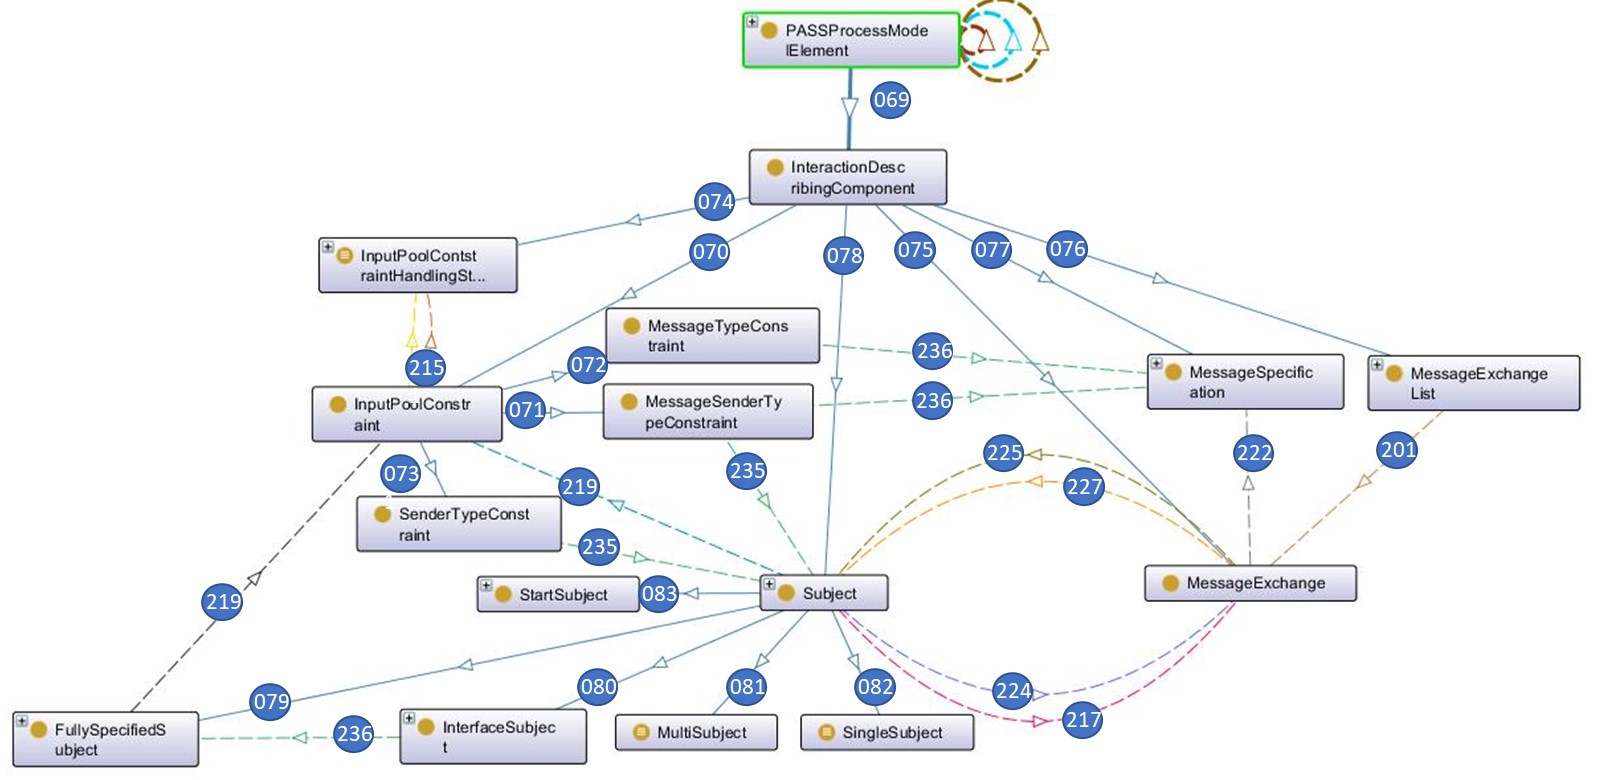
\includegraphics[width=0.9\linewidth]{20181026-Ontologie-Bilder/Grafiken-Ontologie/SUbject-Interaction/20181205-Subject}
	\caption[Subject]{Different Types of Subjects}
	\label{fig:20181205-subject}
\end{figure}

\newpage

\subsection{Messages}

SDescription of messages \ref{fig:20181205-datatypes-payload}

\begin{figure}[ph]
	\centering
	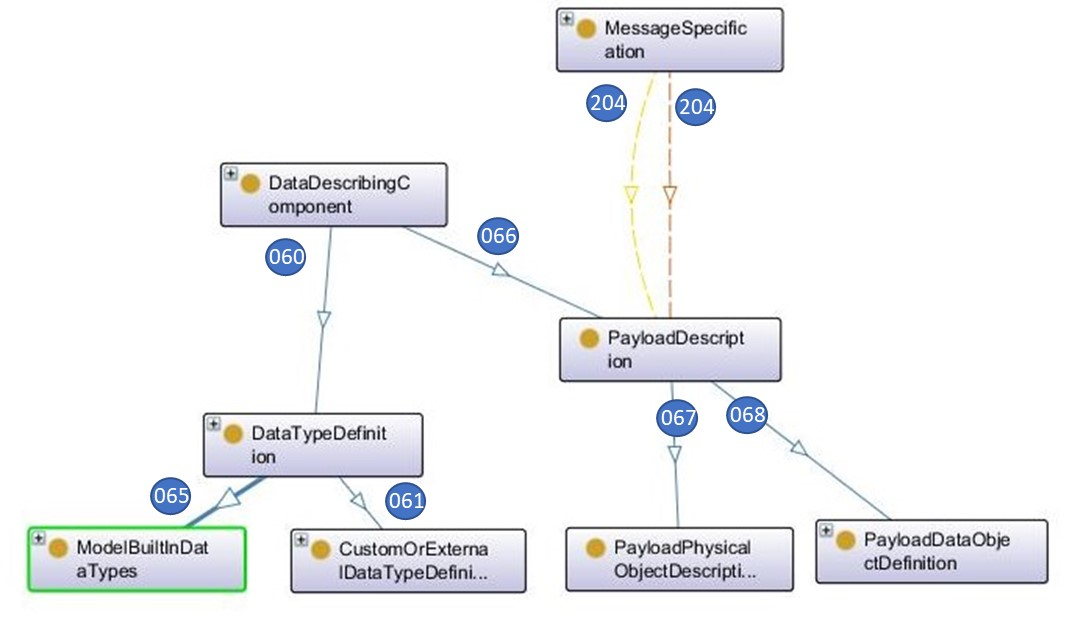
\includegraphics[width=0.7\linewidth]{20181026-Ontologie-Bilder/Grafiken-Ontologie/SUbject-Interaction/20181205-Datatypes-Payload}
	\caption[Message specification]{Message Specification with Payload}
	\label{fig:20181205-datatypes-payload}
\end{figure}

\newpage

\subsection{Input Pools}

Description of input pools \ref{fig:20181203-interaction-describing-component}

\begin{figure}[ph]
	\centering
	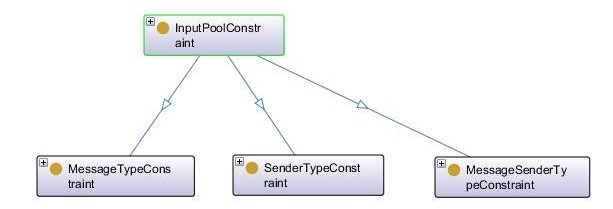
\includegraphics[width=0.7\linewidth]{20181026-Ontologie-Bilder/Grafiken-Ontologie/SUbject-Interaction/input-pool}
	\caption[Input Pool]{Input Pool description}
	\label{fig:input-pool}
\end{figure}



\begin{figure*}[ph]
	\centering
	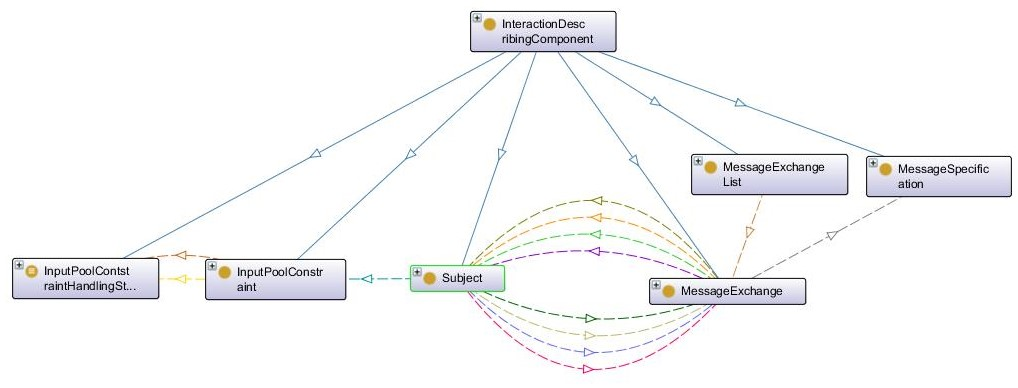
\includegraphics[width=15cm]{20181026-Ontologie-Bilder/Grafiken-Ontologie/SUbject-Interaction/20181203-Interaction-describing-component.jpg}
	\caption[Message Exchange and Input Pools]{Message Exchange and Input Pools}
	\label{fig:20181203-interaction-describing-component}
\end{figure*}


\section{ASM Description}